\subsection{Giới thiệu}
Content-based recommendation system tuy có thể xây dựng mô hình cho mỗi user không phụ thuộc vào các user khác mà chỉ phụ thuộc vào profile của các item thì vẫn còn những nhược điểm là không tận dụng được thông tin từ các user khác và có lúc không thể xây dựng được profile cho mỗi item. Tiếp theo sẽ là phương pháp có thể giải quyết được 2 vấn đề này, đó là \gls{CF}.
\newline Phương pháp dự đoán cơ bản của CF là nếu user X và user Y rate n items gần giống nhau, hay có hành vi giống nhau (cùng xem nhiều loại phim, cùng mua nhiều loại sản phẩm, ...) thì sẽ đánh giá hay tương tác (xem, mua,...) với các sản phẩm khác giống nhau. 
\newline Phương pháp CF là dựa trên độ quan tâm của user tới item đã biết trước để có thể dự đoán được item mà user khác thích. Ví dụ, có danh sách gồm m user {u1, u2, ...um} và 1 danh sách n item {i1, i2, ... , im} và mỗi user ui có 1 danh sách các item Iui mà user đó đã rate (xem, mua, ...). Những giá trị này có thể là rating, số lần mua, số lần click, ... 
\newline Phương pháp CF gặp phải nhiều thử thách. Thuật toán CF cần phải có khả năng xử lý với bộ dữ liệu thưa (bộ dữ liệu mà nhiều user, nhiều item nhưng lại ít rating), có thể xử lý được khi số lượng user và item tăng, đáp ứng cho khoảng thời gian ngắn, và nhiều vấn đề khác.
\newline Điểm khác biệt lớn nhất giữa CF và content-based recommendation system là CF chỉ sử dụng rating của user cho item còn content-based recommendation system thì phụ thuộc vào feature của item để dự đoán. Cả 2 phương pháp đều có những giới hạn nhất định. Do vậy một số phương Hybrid CF cũng đã được phát triển như content-boosted CF hay Personality Diagnosis nhằm vượt qua được những giới hạn của mỗi phương pháp.

\subsection{Những vấn đề gặp phải của Collaborative Filtering}
\textbf{Data sparsity (Dữ liệu thưa)}. Trong thực tế, rất nhiều recommendation system phải xử lý 1 lượng item rất lớn. Utility matrix thường vô cùng thưa nên việc tối ưu hiệu năng của recommendation system là rất quan trọng. Đối với vấn đề này, có 1 phương pháp được áp dụng là phương pháp giảm số chiều dữ liệu ví dụ như Singular Value Decomposition (SVD), loại bỏ những user, item không tiêu biểu hay không cần thiết nhằm giảm số chiều của Utility matrix.

\textbf{Cold start}. Khi có user mới hay item mới vào trong hệ thống, chưa từng có lịch sử rating hay tương tác gì của user, item này, việc gợi ý item phù hợp user có thể trở nên khó khăn. Item mới không được recommend nếu không có ai đánh giá và user cũng không nhận được recommend tốt vì chưa có lịch sử rating hay mua bán gì. Giải pháp như Hybrid CF có thể hỗ trợ vấn đề này. Với những item chưa được rating hay mua bao giờ, nếu có được các feature của item, vẫn có thể recommend được cho người dùng. 

\textbf{Scalability}. Khi số lượng user và item tăng quá nhanh, phương pháp CF bình thường sẽ gặp phải vấn đề scalability, yêu cầu tính toán vượt quá mức có thể đáp ứng. Ví dụ như khi có hàng chục triệu user và hàng triệu item thì độ phức tạp của thuật toán CF là O(n) sẽ là quá lớn. Chưa nói đến việc các hệ thống cần phải phản hồi ngay lập tức để đưa ra gợi ý hợp lý. Phương pháp giảm số chiều dữ liệu như SVD có thể dùng để giải quyết vấn đề scalability tuy nhiên vẫn phải trải qua bước matrix factorization. Ngoài ra còn có phương pháp khác như clustering CF, phương pháp này giải quyết vấn đề bằng cách tìm user để đánh giá trong 1 cụm nhỏ có độ tương đồng cao thay vì trên toàn bộ database. 

\textbf{Gray Sheep}. Gray sheep nói đến những user có quan điểm không nhất quán, không tương đồng với nhóm user nào nên không có nhiều giá trị đối với collaborative filtering. Có phương pháp được áp dụng đến giải quyết vấn đề này là lấy trung bình có tỉ lệ của phương pháp content-based và CF. Tỉ lệ của content-based và CF sẽ được xác định tùy theo mỗi user, cho phép hệ thống tối ưu hóa việc kết hợp content-based và CF cho mỗi user, giúp giải quyết vấn đề gray sheep.

\textbf{Shilling Attacks}. Có nhiều trường hợp đánh giá item, họ đưa ra đánh giá rất tốt về item của họ và đánh giá xấu về những item của đối thủ. Để tối ưu được hệ thống CF thì cần tránh được vấn đề này. Phương pháp item-based CF cho thấy bị ít ảnh hưởng bởi shilling attack hơn là user-based CF. Ngoài ra phương pháp hybrid CF cũng là một giải pháp cho shilling attack vì ít bị phụ thuộc vào đánh giá của user khác hơn so với phương pháp CF đơn thuần.

\subsection{Neighbor-based Collaborative Filtering}
\subsubsection{Similarity Computation (Xác định độ giống nhau)}
Việc quan trọng nhất phải làm trong collaborative filtering là xác định được sự giống nhau (similarity) giữa 2 user hay 2 item. Ví dụ trong item-based CF, việc tính toán độ giống nhau giữa item i và item j là đầu tiên cần tìm ra những user đã đánh giá cả 2 item và áp dụng hàm tính toán độ giống nhau. Còn đối với user-based CF, tính toán độ giống nhau giữa 2 user u và user v mà đã cùng rate nhiều item. Những hàm tính toán độ giống nhau có những hàm như cosine similarity, euclidean distance, pearson correlation.
\newline Cosine similarity là hàm được sử dụng nhiều nhất. Công thức của cosine similarity là dưới đây:
\begin{equation}
    similarity = \cos{u_1, u_2} = \frac{u^T_1 u_2}{\|u^T_1\|.\|u_2\|}
\end{equation}
\newline Trong đó $u_{1,2}$ là vector tương ứng với user 1, 2 đã được chuẩn hóa.
\newline Độ similarity (giống nhau) của 2 vector là 1 số trong đoạn [-1, 1]. Giá trị bằng 1 thể hiện hai vector hoàn toàn similar với nhau. Hàm số cos của một góc bằng 1 nghĩa là góc giữa hai vector bằng 0, tức một vector bằng tích của một số dương với vector còn lại. Giá trị bằng -1 thể hiện hai vector này hoàn toàn trái ngược nhau. Điều này cũng hợp lý , tức khi hành vi của hai users là hoàn toàn ngược nhau thi similarity giữa hai vector đó là thấp nhất.

\subsubsection{Chuẩn hóa dữ liệu}
Khi thực hiện tính similarity, ta vẫn cần phải gán 1 giá trị tạm thời nào đó cho những ô rating trống trong Utility matrix. Nếu gán 0 thì không được vì giá trị quá thấp, sẽ giống như user ghét item đó, nếu gán trị trung bình ví dụ như 3 (đối với rating 1 đến 5) thì vẫn có thể gặp vấn đề như sau. Nếu với những user rating khắt khe, thường chỉ rating 1, 2, 3 thì giá trị 3 ở đây có thể là quá cao, còn với user dễ tính, thường rating 3, 4, 5 thì giá trị này là có thể là quá thấp. Do vậy, cần phải chuẩn hóa dữ liệu của Utility matrix.
\newline Bước đầu tiên của chuẩn hóa là tính trung bình các rating của người dùng. Giá trị này cao sẽ tương ứng với user dễ tính và ngược lại. Tiếp tục trừ từ mỗi rating đi giá trị này và thay giá trị chưa biết bằng không thì ta được Utility matrix đã chuẩn hóa. Bước chuẩn hóa này quan trọng cũng vì lý do sau đây. Thứ nhất, việc trừ đi trung bình cộng của mỗi cột khiến trong trong mỗi cột có những giá trị dương và âm. Những giá trị dương tương ứng với việc user thích item, những giá trị âm tương ứng với việc user không thích item. Những giá trị bằng 0 tương ứng với việc chưa xác định được liệu user có thích item hay không. Lý do thứ hai là vì số chiều của Utility matrix thường rất lớn, có thể lên tới hàng chục triệu user và hàng triệu item, việc lưu toàn bộ Utility matrix sẽ tốn rất nhiều bộ nhớ. Thấy rằng số lượng rating biết trước thường rất nhỏ so với kích thước của utility matrix nên cách tốt hơn là lưu dưới dạng sparse matrix, tức chỉ lưu giá trị khác không và vị trí của chúng. Tức là những rating chưa biết nên được thay bằng 0. Việc này giúp tối ưu bộ nhớ rất nhiều.

\subsubsection{Điền các giá trị khuyết trong utility matrix}
Việc dự đoán mức độ quan tâm (predict rating) của user với một item dựa trên các user giống với user này nhất rất giống với phương pháp k-nearest neighbors (KNN) với hàm khoảng cách là cosine similarity. Tương tự như KNN, neighbor-based CF cũng dùng thông tin của k user gần nhất để dự đoán. Để đánh giá độ quan tâm của user đối với 1 item, chỉ cần quan tâm tới các user lân cận đã từng đánh giá item đó. Tuy nhiên, trong KNN thì các distance là các khoảng cách không âm còn similarity trong neighbor-based thì có thể âm. Công thức dự đoán rating của user u cho item i là:
\begin{equation}
    \widehat{y_{i,u}} = \frac{\sum_{u_j \in N(u,i)} \overline{y_{i,u}} sim(u,u_j)}
                        {\sum_{u_j \in N(u,i)} |sim(u,u_j)|}
\end{equation}
Trong N(u, i) là tập hợp k user có similarity cao nhất với user u mà đã rate i.
Để quy đổi giá trị rating dự đoán về thang 5, cộng giá trị dự đoán với giá trị rating trung bình của mỗi user.
\newline Việc thực hiện recommend có thể thực hiện theo nhiều cách. Có thể sắp xếp những item chưa được rate theo giá trị giảm dần của rating dự đoán để recommend cho người dùng, hoặc recommend tất cả item có rate dự đoán đã chuẩn hóa lớn 0.

\subsubsection{Item-based collaborative filtering}
Phương pháp user-based vẫn còn 1 số hạn chế như sau. Đầu tiên là, số lượng user thường lớn hơn số lượng item rất nhiều. Do đó kích thước ma trận similarity là rất lớn. Việc lưu trữ ma trận nhiều khi không khả thi. Thứ hai là, utility matrix thường rất sparse và số lượng user lại rất lớn so với số lượng item dẫn đến nhiều cột của utility matrix có rất ít hoặc không có giá trị biết trước. Do đó, khi user thay đổi rating trước đó hay đánh giá thêm item, trung bình cộng rating hay vector chuẩn hóa thay đổi rất nhiều. Dẫn đến việc tính toán ma trận similarity, vốn đã tốn nhiều thời gian và bộ nhớ, cần phải thực hiện lại.
\newline Cách tiếp cận khác là thay vì tìm sự giống nhau giữa các user, chuyển sang tìm sự giống nhau giữa các item. Nếu user thích 1 item thì hệ thống nên gợi ý những item tương tự item đó cho user đó. Phương pháp này có những ưu điểm sau. Vì số item nhỏ hơn nhiều số item nên ma trận similarity nhỏ hơn rất nhiều giúp tính toán hiệu quả hơn. Thứ hai là vì số lượng item ít hơn user mà tổng rating không đổi, dẫn đến việc số rating item có được sẽ nhiều hơn số rating mà user rate. Từ đó dẫn đến việc tính độ similarity đáng tin cậy hơn, giá trị trung bình mỗi hàng thay đổi ít hơn khi có rating bị thay đổi dẫn tới việc cập nhật ma trận similarity được thực hiện ít hơn.

\subsubsection{Top-N recommendation}
Top-N recommendation là việc recommend 1 tập hợp gồm N item được xếp hạng mà user có thể thích. Ví dụ như khi sử dụng youtube, nếu user truy cập youtube với tài khoản youtube của mình, ở trang chủ, user sẽ được recommend 1 số video phù hợp với mỗi cá nhân. Phương pháp Top-N recommendation phân tích utility matrix để tìm ra sự liên hệ giữa các user hay item khác nhau và dựa trên đó tìm những gợi ý hợp lý. Ta có thể chia Top-N recommendation thành 2 phương pháp là user-based top-N recommendation và item-based top-N recommendation.
\newline Với phương pháp user-based top-N recommendation, bước đầu tiên là tìm ra k user giống nhất với user đang muốn được recommendation nhất. Sau khi đã tìm ra k user đó, những item đã được k user này đánh giá (mua, xem) được tập hợp thành 1 tập C. Trong tập C, những sản phẩm được rating cao hay xuất hiện nhiều mà user chưa mua sẽ được ưu tiên recommend.
\newline Còn với phương pháp item-based top-N recommendation, đầu tiên tìm tập k item giống nhất với mỗi item mà user đã mua. Sau đó tìm ra tập C bằng cách loại bỏ những item mà user đã mua ra khỏi tập k item giống nhất với các item đã mua. Những item còn lại sẽ được xếp hạng dựa trên độ giống của item với item mà người dùng đã mua.

\subsubsection{Lợi thế và khó khăn khi ứng dụng neighbor-based collaborative filtering}
Việc ứng dụng neighbor-based CF có những lơi thế khá rõ như dễ áp dụng, không phụ thuộc vào thông tin của item, không phải thực hiện công đoạn huấn luyện, ngoài ra so với phương pháp khác như content-based thì có độ chính xác cao hơn.

Tuy nhiên, phương pháp neighbor-based CF vì là phương pháp memory-based nên vẫn có vấn đề lớn về khả năng mở rộng (scalability). Khi mà số người dùng hay số item trở nên quá lớn, ma trận similarity sẽ tốn rất nhiều bộ nhớ. Hơn nữa, với số user hay item càng lớn thì việc tìm ra K hàng xóm gần nhất sẽ có cost rất lớn,

\subsection{Clustering collaborative filtering}
\subsubsection{Model-based CF}
Phương pháp neighbor-based CF ở trên là phương pháp memory-based CF. Phương pháp Memory-based CF sử dụng toàn bộ hay một phần của bộ dữ liệu để thực hiện việc dự đoán. Phương pháp này có một số ưu điểm như là dễ áp dụng, data mới có thể dễ dàng được thêm vào và sử dụng luôn để đánh giá. Tuy vậy memory-based CF vẫn còn một số nhược điểm như hiệu suất thâm khi bộ dữ liệu thưa và đặc biệt là ít có khả năng mở rộng quy mô khi gặp bộ dữ liệu quá lớn do tốn rất nhiều bộ nhớ. Những vấn đề này có thể được giải quyết với Model-based CF. Clustering CF là 1 trong những phương pháp tiếp cận của Model-based CF.

\subsubsection{Giới thiệu Clustering CF}
\noindent Nội dung dưới đây được đươc viết dựa theo tài liệu \cite{locnguyen2010modelbased}.
\newline Clustering \gls{CF} là hướng tiếp cận dựa trên bài toán phân tích ma trận thành phân tử (matrix factorization hoặc matrix decomposition). Clustering \gls{CF} dựa trên giả định rằng người dùng trong cùng một nhóm có cùng sở thích, vì vậy những người dùng này đánh giá các mặt hàng tương tự nhau. Do đó, người dùng được phân chia thành các nhóm được gọi là các cluster được định nghĩa là một nhóm người dùng tương tự nhau.
\newline Giả sử mỗi người dùng được biểu diễn dưới dạng vector xếp hạng ký hiệu $u_i$ = ($r_{i1}$, $r_{i2}$,..., $r_{in}$). Thước đo khác nhau giữa hai người dùng là khoảng cách giữa họ. Chúng ta có thể sử dụng khoảng cách Minkowski, khoảng cách Euclidian khoảng cách Manhattan hay độ tương đồng cosine.
$$ distance_{Minkowski}(u_1,u_2) = \sqrt[q]{\underset{j}{\sum}(r_{1j} - r_{2j})^q} $$
$$ distance_{Euclidian}(u_1,u_2) = \sqrt{\underset{j}{\sum}(r_{1j} - r_{2j})^2} $$
$$ distance_{Manhattan}(u_1,u_2) = \underset{j}{\sum}|r_{1j} - r_{2j}| $$
$$ similarity_{cosine} (u_1,u_2) = \cos{u_1, u_2} = \frac{u^T_1 u_2}{\|u^T_1\|.\|u_2\|} = \frac{\underset{j}{\sum}r_{1j} r_{2j}}{\sqrt{\underset{j}{\sum}r_{1j}^2} \sqrt{\underset{j}{\sum}r_{2j}^2}} $$

Khoảng cách giữa $u_1$ và $u_2$ càng ngắn hay độ tương đồng càng cao thì $u_1$ và $u_2$ càng giống nhau. Để thực hiện Clustering \gls{CF} cần thực hiện 2 bước sau:
\begin{itemize}
    \item Phân người dùng thành các cụm và mỗi cụm luôn chứa các giá trị đánh giá. Ví dụ, Mỗi cụm đều là kết quả từ thuật toán k-mean và một giá trị trung bình là vector đánh giá giống như vector người dùng.
    \item Người dùng cần được gợi ý được đưa vào một trong các cụm và đánh giá của người đó sẽ giống như đánh giá của cụm đó. Việc đưa người dùng vào cụm nào sẽ dựa trên khoảng cách của người dùng đới với cụm.
\end{itemize}
Vây nên bước quan trọng nhất là làm sao để phân người dùng vào các cụm. Có nhiều phương pháp clustering như k-mean và k-centroid. Phương pháp phổ biến nhất là k-mean, bao gồm 3 bước sau đây:
\begin{itemize}
    \item Ta chọn ngẫu nhiên k người dùng, mỗi người ban đầu đại diện cho tâm của một cụm. Từ đó, chúng ta có k tâm cụm. Mỗi tâm cụm này được coi là đại diện của người dùng của một cụm. Có tổng cộng k cụm.
    \item Đối với mỗi người dùng, khoảng cách giữa mỗi người dùng với k tâm cụm được tính toán. Người dùng đó sẽ thuộc về cụm gần nhất. Nói cách khác, nếu người dùng $u_i$ thuộc về cụm $c_v$, khoảng cách giữa $u_i$ và tâm $m_v$ của cụm $c_v$, được ký hiệu là $distance(u_i, m_v)$ là nhỏ nhất trong tất cả các cụm.
    \item Sau đó, tâm của tất cả các cụm được tính toán lại. Nếu điều kiện dừng được thỏa mãn thì dừng lại, nếu không thì lặp lại bước thứ 2.
\end{itemize}
Quá trình này được lặp lại cho đến khi điều kiện dừng được thỏa mãn. Có hai điều kiện dừng điển hình cho thuật toán k-mean:
\begin{itemize}
    \item k tâm của các cụm không thay đổi. Nói cách khác, k cụm không thay đổi. Điều kiện này thể hiện đã hoàn thành phân cụm.
    \item Cách khác là tiêu chí lỗi nhỏ hơn một ngưỡng được xác định trước.
\end{itemize}
Nếu như điều kiện dừng là tiêu chí lỗi nhỏ hơn một ngưỡng được xác định trước, tiêu chí lỗi sẽ được tính nhau sau:
$$ error = \underset{v=1}{\overset{k}{\sum}} \underset{u_i \in c_v}{\sum} distance(u_i,m_v) $$
Trong đó $c_v$ và $m_v$ lần lượt là cụm v và tâm của nó.

\subsubsection{Lợi thế và vấn đề gặp phải khi áp dụng Clustering Cf}
Phương pháp clustering CF có lợi thế như có thể dễ dàng áp dụng để chia bộ dữ liệu phức tạp thành nhiều cụm khác nha;, phù hợp cho bộ dữ liệu lớn; có tính linh hoạt cao, điều chỉnh tâm các cụm có thể thay đổi kết quả đầu ra; có thời gian chạy tuyến tính với số đối tượng.

Tuy nhiên clutering CF còn có một số vấn đề như không thể biết được số lượng cụm tối ưu do đó số cụm phải được chọn từ trước; nếu các cụm ban đầu được chọn ngẫu nhiên thì kết quả có thể thiếu tính nhất quán.

\subsection{Matrix factorization collaborative filtering}
\noindent Nội dung dưới đây được đươc viết dựa theo tài liệu \cite{machinelearningbasic}.
\subsubsection{Giới thiệu}
\gls{MFCF} là một hướng tiếp cận khác cho collaborative filtering dựa trên bài toán phân tích ma trận thành nhân tử (matrix factorization hoặc matrix decomposition). 

Trong content-based recommendation system, mỗi item đều có item profile, được mô tả bằng vector $x$. Ta cần tìm vector hệ số $w$ tương ứng với mỗi người dùng. Từ đó đánh giá của người dùng đó cho item xấp xỉ với:
$$ y \approx w^T x = x^T w $$
Khi đó ma trận utility sẽ xấp xỉ với:
$$ Y \approx X^T W $$
Trong content-based recommendation system, vector x được xây dựng dựa trên thông tin của item. Như vậy việc xây dựng item profile đóng vai trò quan trọng, ảnh hưởng trực tiếp đến hiệu năng của mô hình.

Giả sử, không cần phải xây dựng trước các vector x dựa trên thông tin item và vector này có thể được huấn luyện đồng thời với vector hệ số của mỗi người dùng. Có nghĩa là biến số trong bài toán tối ưu là cả X và W. X là man trận của toàn bộ item profile, mỗi cột tương ứng với một item, W là ma trận của toàn bộ vector hệ số của người dùng, mỗi cột tương ứng với một người dùng.

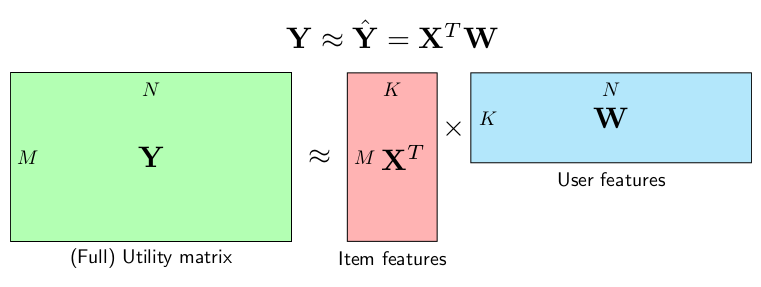
\includegraphics[width=\textwidth]{thesis/images/MFCF1.png}

Với cách làm này, ta cố gắng xấp xỉ ma trận utility $Y \in R^{M \times N}$ bằng tích của hai ma trận $ X \in R^{M \times K} $ và $ W \in R^{K \times N} $. Thông thường, K được chọn là số nhỏ hơn rất nhiều so với M, N. Khi đó, cả hai ma trận X và W đều có rank không vượt quá K. Do vậy, phương pháp này còn được gọi là low-rank matrix factorization. 

Ý tưởng đằng sau \gls{MFCF} chính là sự tồn tại của các tính chất ẩn mô tả sự liên quan giữa các item và người dùng. Ví dụ trong hệ thống gợi ý sách, những tính chất ẩn ở đây có thể là các thể loại sách trinh thám, lịch sử, giáo dục,... hoặc cũng có thể là kết hợp nào đó của các thể loại này. Mỗi item sẽ mang tính chất ẩn ở một mức độ nhất định nào đó, điều này sẽ được thể hiện ở vector x của item đó, hệ số này càng cao thể hiện item mang cần nhiều tính chất đó. Mỗi người dùng cũng tương tự như vậy. Mỗi người dùng có thể có sở thích đọc sách trinh thám, lịch sử, giáo dục,... hoặc thích thể loại được kết hợp bởi những thể loại này, điều này sẽ được thể hiện ở vector w của người dùng đó. Hệ số của 1 tính chất ẩn nào đó càng cao càng chứng tỏ người dùng càng thích item chứa nhiều tính chất ẩn đó. Từ đó giá trị $x^T w$ sẽ thể hiện được hứng thú của người dùng với item nhất định. Hệ số tính chất ẩn của item càng lớn và hệ số thể hiện độ thích của người dùng với tính chất đó càng lớn, giá trị trên sẽ càng lớn.